%!TEX root = ../template.tex
%%%%%%%%%%%%%%%%%%%%%%%%%%%%%%%%%%%%%%%%%%%%%%%%%%%%%%%%%%%%%%%%%%%%
%% chapter4.tex
%% NOVA thesis document file
%%
%% Chapter with lots of dummy text
%%%%%%%%%%%%%%%%%%%%%%%%%%%%%%%%%%%%%%%%%%%%%%%%%%%%%%%%%%%%%%%%%%%%

\typeout{NT FILE chapter4.tex}%

\chapter{Results}
\label{cha:results}

\section{Benchmark platform} % (fold)
\label{sec:benchmark_platform}

We plan to construct a benchmark platform to compare our solution to existing ones; this section discusses the proposed benchmark platform's requirements and design.

\begin{figure}[htbp]
    \centering
    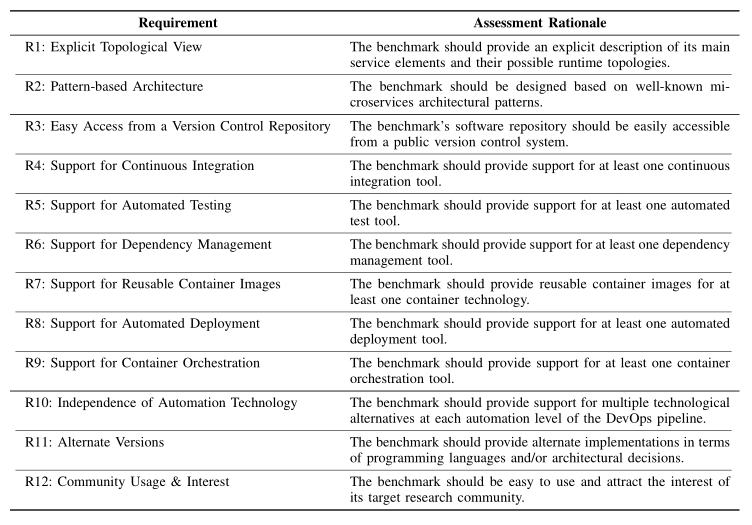
\includegraphics[height=4in]{benchmark_requirements}
    \caption{Benchmark Requirements \cite{microservices2017benchmark}}
    \label{fig:benchmark}
\end{figure}

\citeauthor{microservices2017benchmark} propose an initial set of requirements
to support repeatable microservices research.
In addition to the requirements listed in the ~\ref{fig:benchmark}, the platform's essential requirements are as follows:
\begin{itemize}
    \item The ability to evaluate different solutions in comparable scenarios while utilizing the same evaluation criteria.
    \item Evaluating solutions without requiring modifications to implementations.
    \item Experiments must be simple to share and reproduce by different individuals.
    \item It should be possible to aggregate reported metrics for a specific time period between two events, such as the start and end of a service's evolution.
    \item Users must be able to specify how and when each service should evolve via a configuration file or directly through a terminal.
\end{itemize}

The architecture of the benchmark platform can be seen in section ~\ref{fig:canvas}.
The architecture components, and their applications are described below:

\paragraph{Kubernetes ~\cite{kubernetes}} will be the test environment.
It will host the services holding the solutions implementations.
The loading testing scripts will also be managed via services in Kubernetes.

\paragraph{Promotheus ~\cite{turnbull2018monitoring}} is a pull-based monitoring system.
It periodically sends HTTP scrape requests, the response to this requests is parsed in storage along with the metrics for the scrape itself.
Prometheus provides a query language that allows the metrics to be aggregated by events, components or metadata.
The gathered will be visualized in this platform via Grafana dashboards.

\paragraph{Artillery}

\paragraph{Jenkins}

\begin{figure}[htbp]
    \centering
    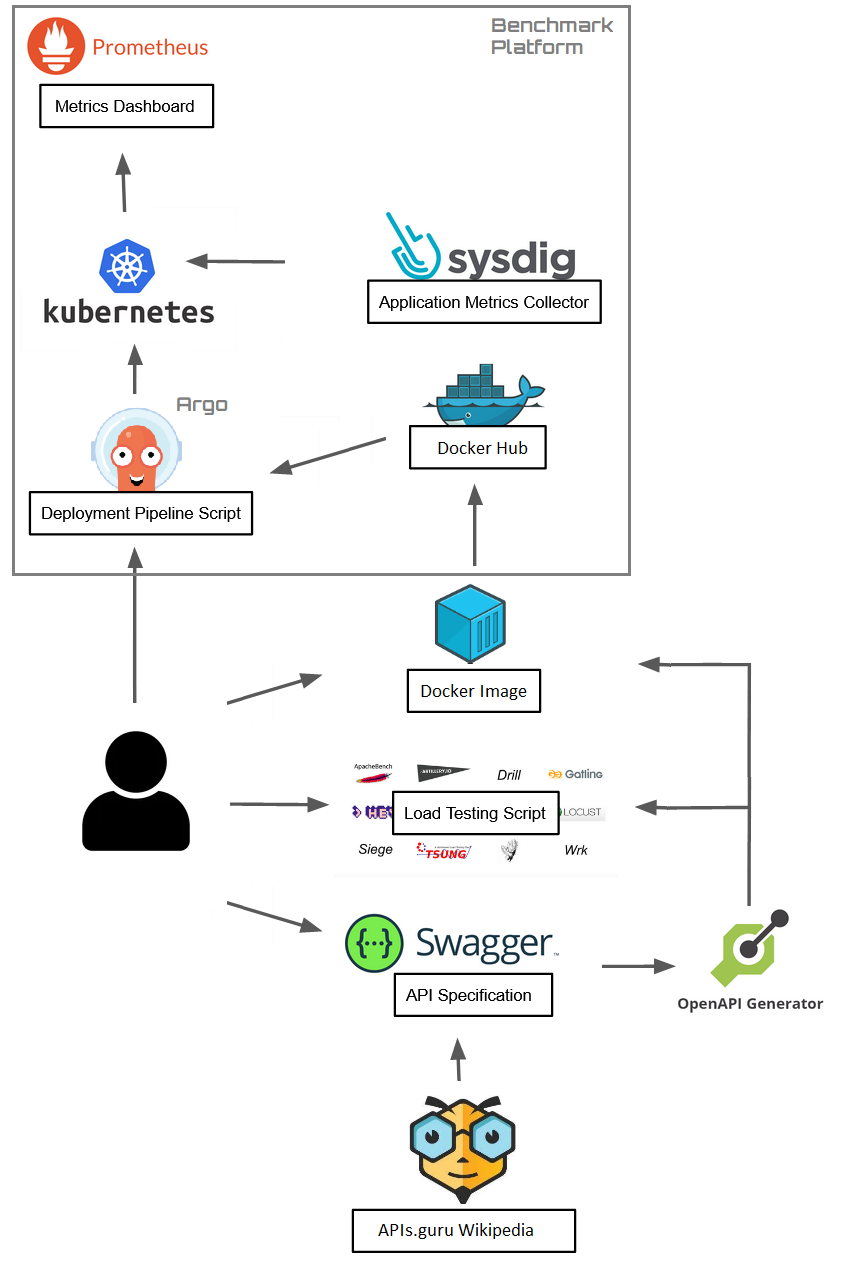
\includegraphics[height=7in]{canvas}
    \caption{Benchmark platform components}
    \label{fig:canvas}
\end{figure}

\section{Evaluation Methodology} % (fold)
\label{sec:evaluation_methodology}

\paragraph{Environment}

The experiments were conducted in a cloud environment with 10 virtual machines.
All 10 nodes were hosted in the same datacenter in the region of Strasbourg, France.
Each virtual machines was hosted in different physical machines, no two VMs shared the same hardware.
Each node is interconnected with a bandwidth of 2 Gb/s.
Each virtual machine is equipped with 4GB of RAM and 2 virtual cores of an Intel Core Haswell (no TSX) cpu.

\paragraph{Tested microservice system }

To test the cost of the adapter system a demo application was developed.
The demo application holds a configurable amount of services that run an identical image.
The image is a simple http spring server that returns received requests unchanged.
The interconnections between microservices is configurable thorough environment variables.
The number of synchronous calls (SyC) between microservices for a single request is also configurable.
The number of parallel calls (PrC) between microservices is also configurable.
Two http endpoints are contained in the image, which was developed in two separate versions with unique contracts.
In one of the endpoints, all the parameters in the body's schema were given new names.

\paragraph{Experiment Setup}

To inject load in the experiments, 10 workers of artillery load testing tool were used,
the workers are executed remotely in the cluster and were spread in 6 nodes.
The workers are supported by kubernetes pods that are monitored by a common kubernetes job.
The workers are installed and removed from cluster using the artillery operator project, that enables
the creation and execution of distributed Artillery load tests from a Kubernetes cluster, at scale.
In each experiment all the resources of previous experiments were deleted and a new job and namespace were created in the
cluster to avoid contamination in the metrics extracted.
Each experiment was executed in sequence with a pause of 2m.

Each experiment had three phases:
A warm up phase of 30s with an arrival rate of 5 vu/s.
A ramp up phase of 2m.
A sustained load phase of 6m.
The metrics were only extracted during the sustained load phase;
the first and last 30s were left out to allow time for all the artillery worker threads to enter the sustained load phase.
We excluded tests that had a high enough throughput to saturate the application.
The error rate and timeouts were zero during all the presented experiments.

\begin{figure}[htbp]
    \centering
    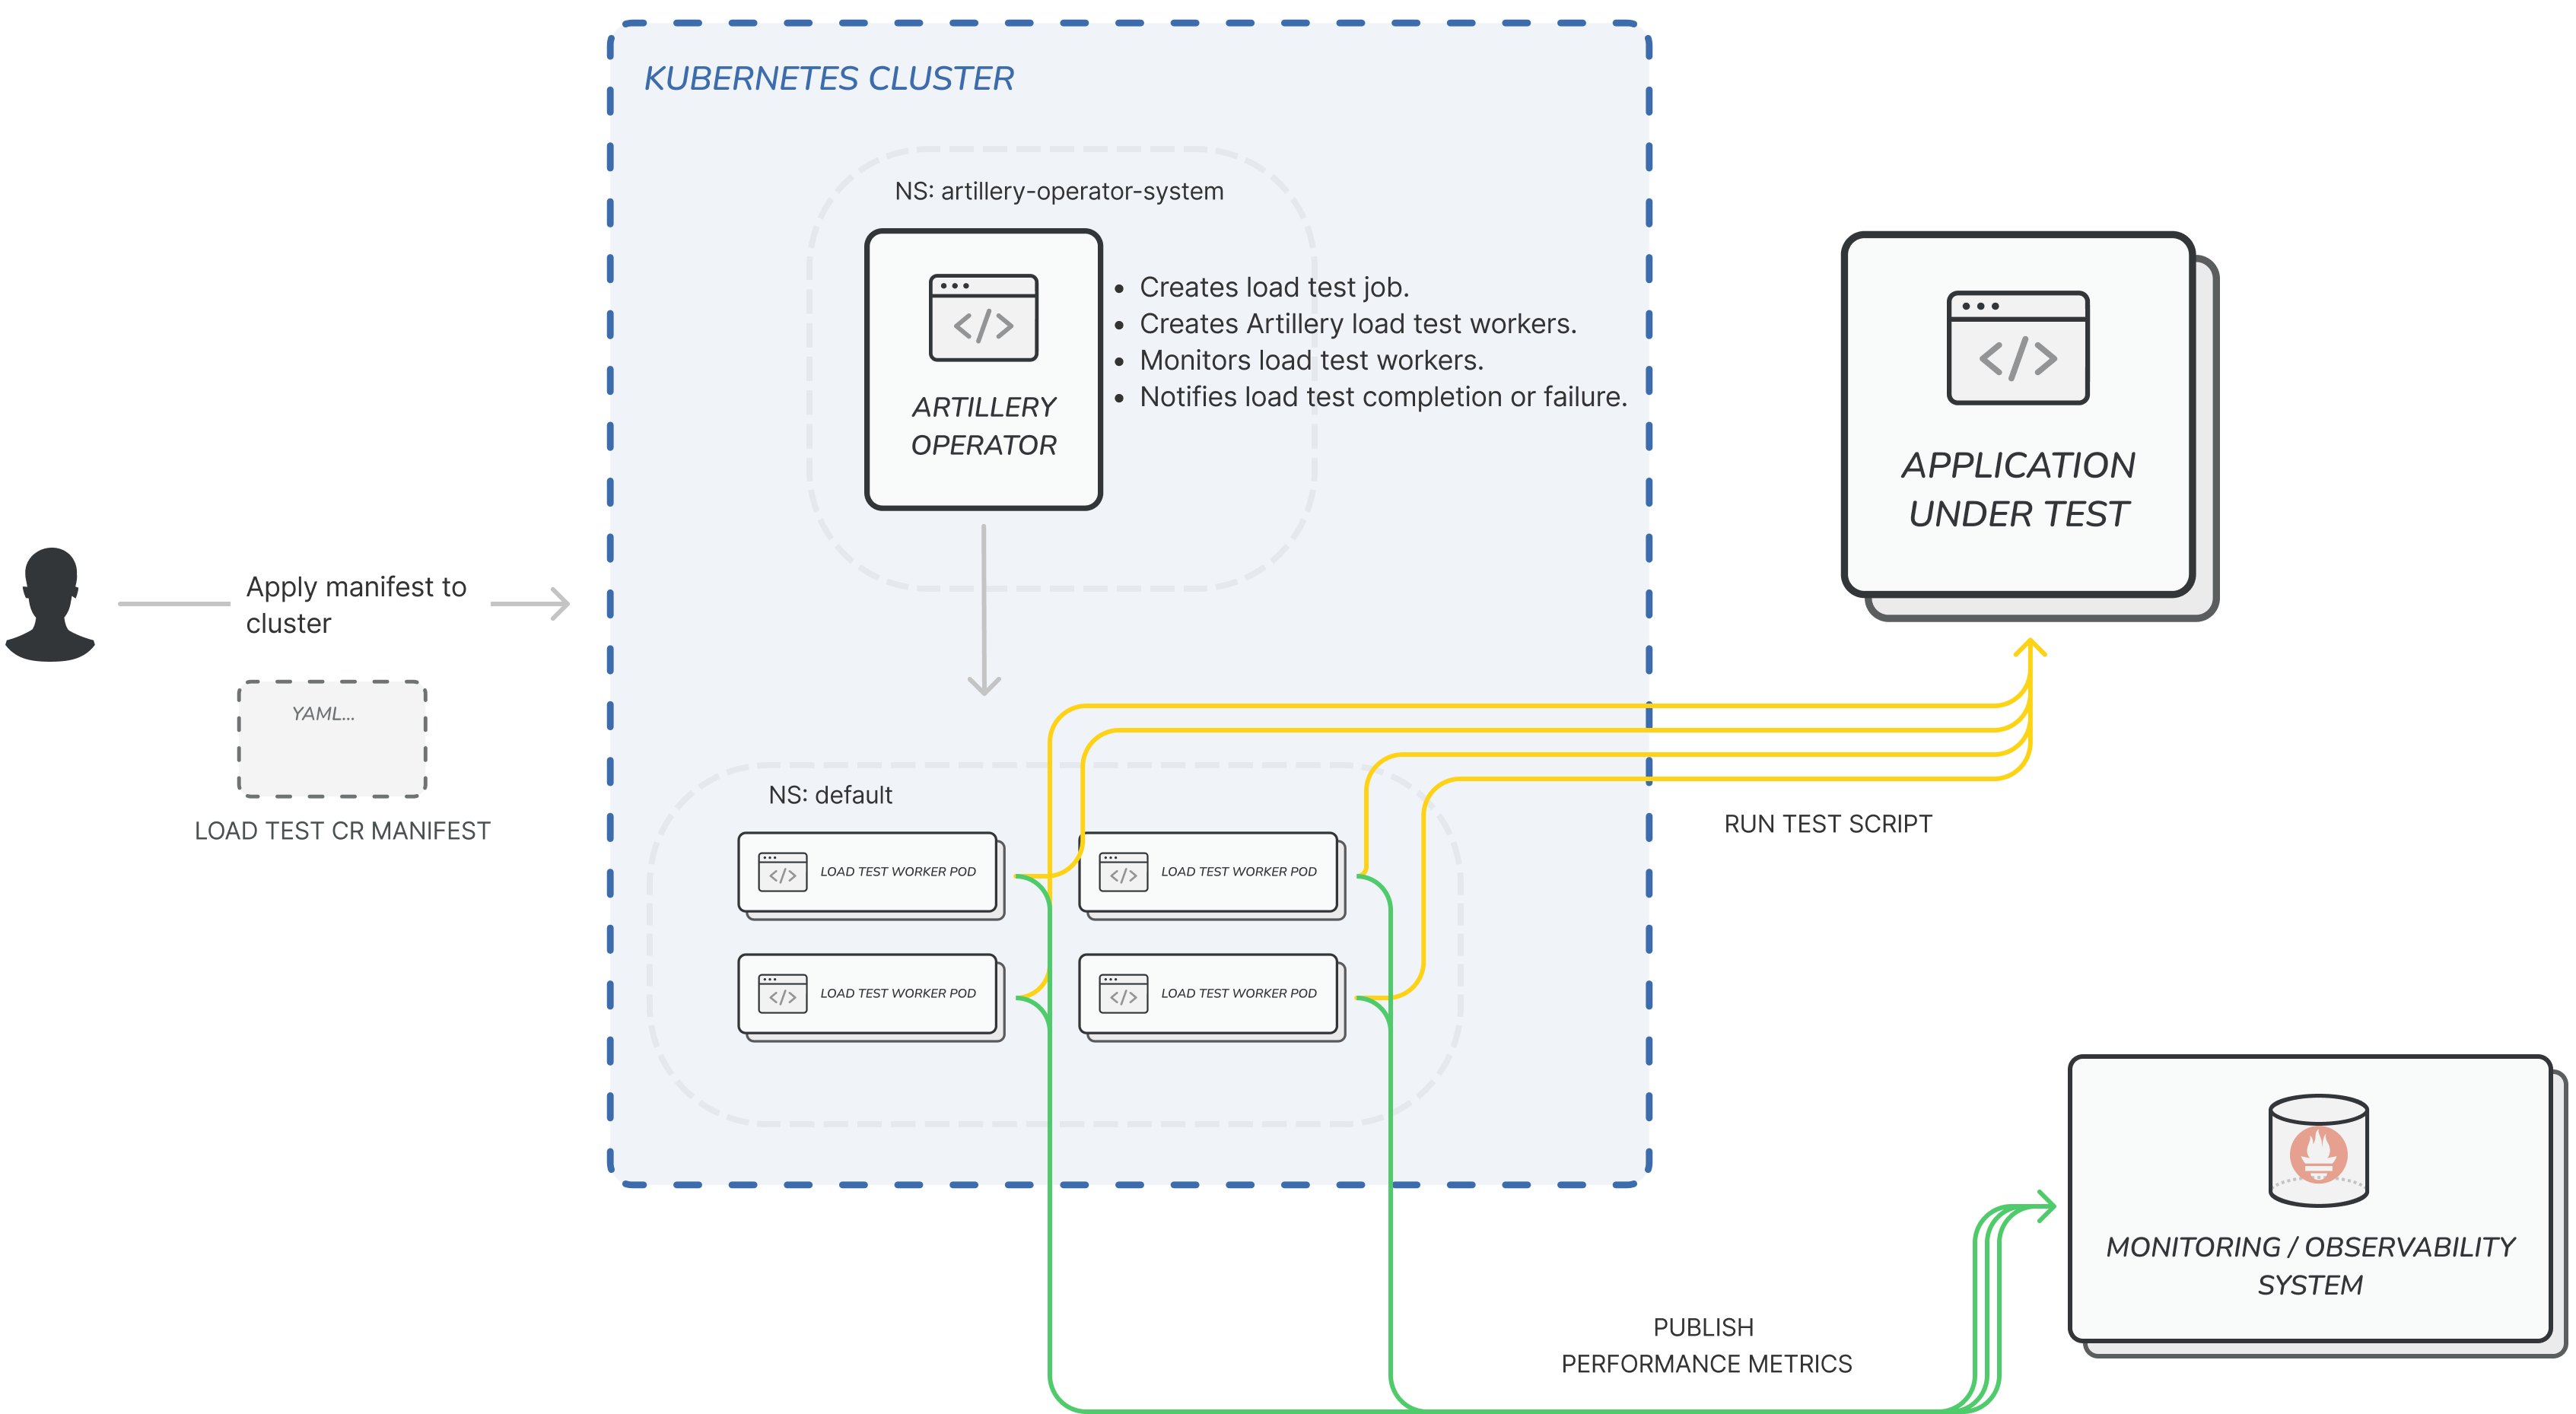
\includegraphics[height=3in]{artillery-operator-architecture}
    \caption{Artillery Operator Architecture}
    \label{fig:gantt}
\end{figure}

\paragraph{Metrics}

In each experiment we extracted 3 metrics, the cpu/memory resources and latency of the system.
The resources were only queried from the adapters, and the replicas that belong to the target microservice application.
The resources consumed by the monitoring system and artillery workers were excluded and have no effect
on the results.
The throughput and latency were extracted with the use of the artillery load testing tool.

The CPU resource samples were taken from each node at 5-second intervals using the prometheus node exporter.
Memory resource samples were gathered from each container at 5-second intervals using the kubelet node agent api.
The latency statistics were calculated with a period of 10s over 5 min, the results obtained represent the
average of the reported 30 periods.

\section{Experiments} % (fold)
\label{sec:experiments}

This section presents measurements obtained from a prototype implementation throughout various experiments.

%%Throughout the experiments, if the behavior of the system is similar with different parameters, we select the most
%%interesting figures or features due to the limited space.

\paragraph{Point to Point}

\begin{figure}[htbp]
    \centering
    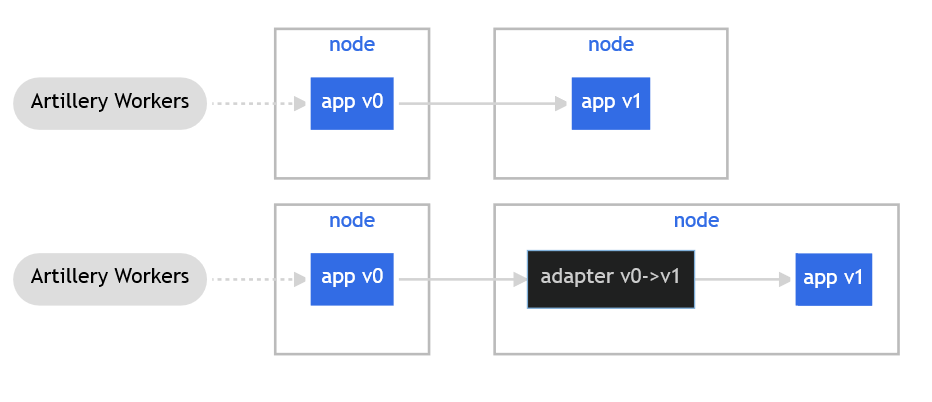
\includegraphics[height=2.4in]{pointExperiment}
    \caption{point-to-point experiment}
    \label{fig:point}
\end{figure}

The topology of this experiment is represent in Figure ~\ref{fig:point}.
This experiment is composed by two microservices:
the first receives requests from artillery workers and forwards them to the second microservice, which responds with the request.

We first established a baseline of comparison
by doing the tests without the adapter, and then we introduced the adapter and repeat the tests.
The primary goal of this experiment was to assess the overhead of the adapter in terms of latency and computational resources.

\paragraph{}

The measured cpu overhead of the adapter over a
range of request rates is depicted in Figure ~\ref{fig:cpuPtp}.
The overhead was calculated by processing the averages of the measured CPU resources in the baseline and adapter tests, and then by dividing the two averages.

In this experiment it is expected to have an overhead of 150\%, because the adapter and the microservices share the same request rate,
and because the cost of the adapter is expected to be equal or to the cost of the tested microservices.
The tested microservices were implemented with the same frameworks as the adapter, consequently adding the adapter will be equivalent to adding one more microservice to the existing two.

As can be seen in the results shown Figure ~\ref{fig:cpuPtp} the measured overhead doesn't fall to far outside our expectations, with the exception of the first data point.
The overhead 84\% is explainable by the configuration of the containers.
The adapter and demo application containers were initialized in kubernetes with a default of 100 millicpu (10\% of tested cpu core),
this cpu resources far exceed the capacity necessary to support a request rate 60 requests/second,
consequently the container's cpu scheduling was throttle-down after start up,
the overhead was inferior to 100\% because the scheduled cpu resources in the experiment with the adapter, were throttled down faster than in the baseline experiment without the adapter.

\paragraph{}

Figure ~\ref{fig:memPtp} shows the measured memory overhead of the adapter over a
range of request rates.
The average cost of 190\% in Figure ~\ref{fig:memPtp} is understandable because, although being stateless, the adapter stores two messages in memory for each request, the request message and the adapted request message.
Because the demo application only keeps one request in memory, it stands to reason that the adapter memory cost is the double of the demo application.
As can be seen in Figure ~\ref{fig:memCostPtp} the adapter real memory cost grows linearly with the request rate.


\begin{figure}[htbp]
    \centering
    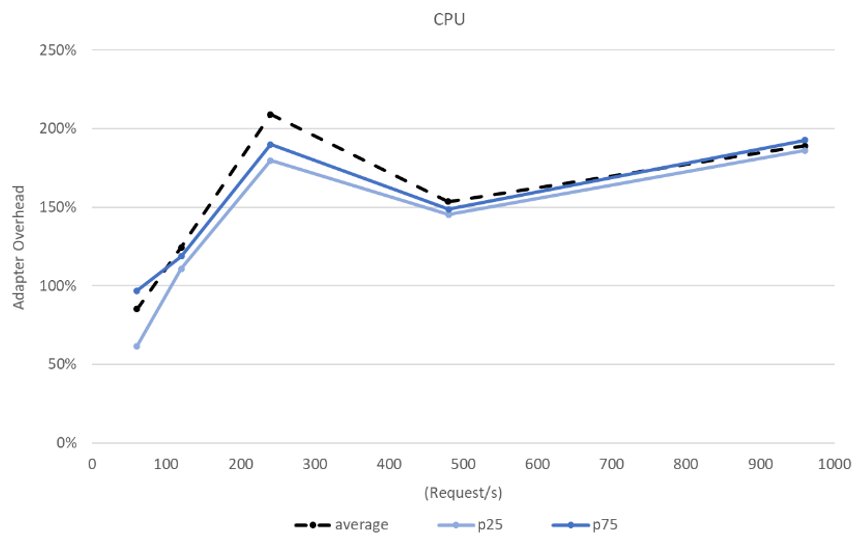
\includegraphics[height=3in]{Results/PtP/Cpu-PtP}
    \caption{Adapter CPU overhead in the point-to-point experiment \\\hspace{\textwidth} 100 bytes (payload size)}
    \label{fig:cpuPtp}
\end{figure}

\begin{figure}[htbp]
    \centering
    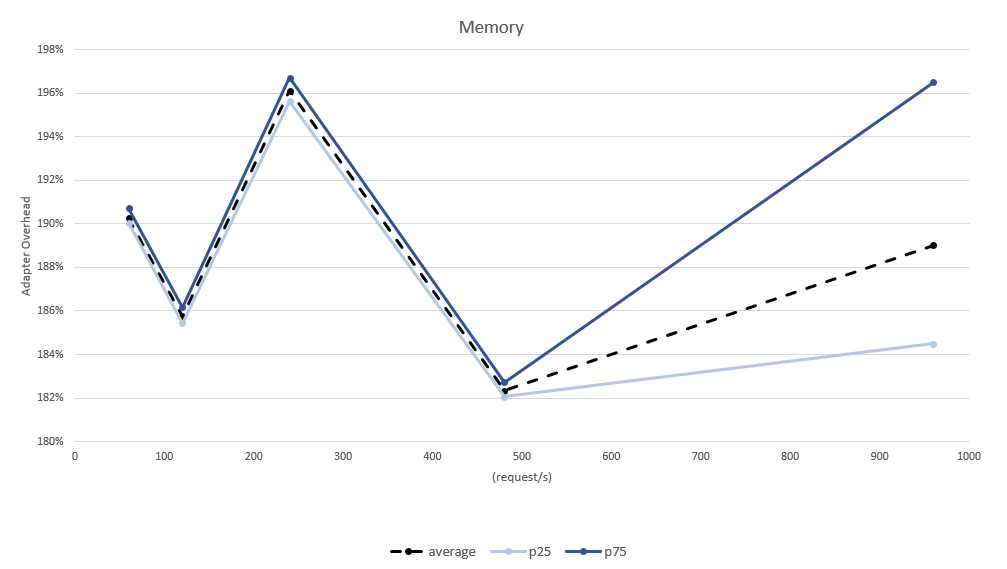
\includegraphics[height=3in]{Results/PtP/Memory-PtP}
    \caption{Adapter memory overhead in the point-to-point experiment \\\hspace{\textwidth} 100 bytes (payload size)}
    \label{fig:memPtp}
\end{figure}

\begin{figure}[htbp]
    \centering
    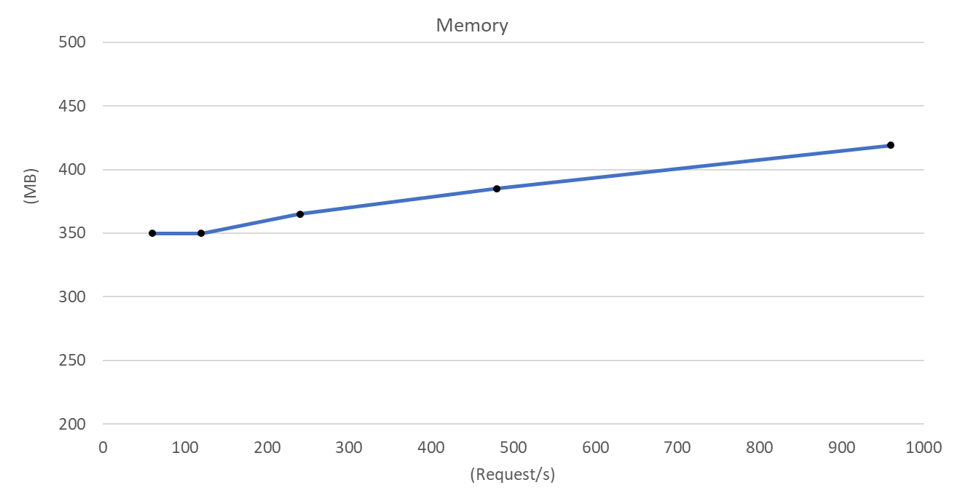
\includegraphics[height=3in]{Results/PtP/MemoryCost_PtP}
    \caption{Adapter memory cost in the point-to-point experiment \\\hspace{\textwidth} 100 bytes (payload size)}
    \label{fig:memCostPtp}
\end{figure}

\newpage

The latency overhead of the adapter in the point-to-point experiment is depicted in Figure ~\ref{fig:latPtP}.

It is expected for the overhead to be less or equal to 150\%, because the latency overhead is largely attributable to communication cost.
The adapter introduces an additional communication step "app1->\textbf{adapter->app2}" to the baseline communication chain that already haves two steps "workers->app1" and "app1->app2".
The introduced communication step is expected to have a slightly inferior cost to the other steps, because it is performed via interprocess-calls, while the others are done via a private network with 2 GB of bandwidth.
Our hypothesis is confirmed by the experiment results in Figure ~\ref{fig:latPtP}.

\begin{figure}[htbp]
    \centering
    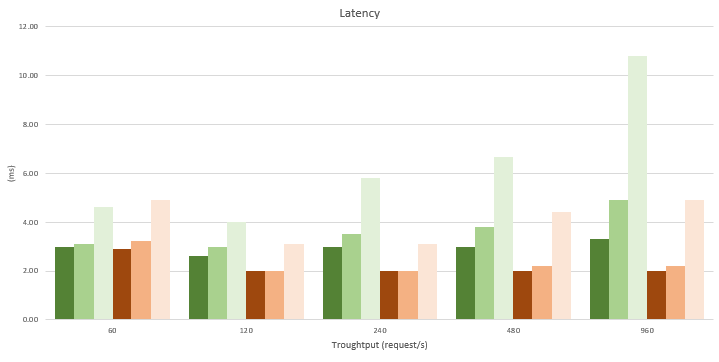
\includegraphics[height=3in]{Results/PtP/Latency-PtP}
    \caption{Adapter latency cost in the point-to-point experiment \\\hspace{\textwidth} 100 bytes (payload size)}
    \label{fig:latPtP}
\end{figure}

The Figures  ~\ref{fig:payloadCpuPtP} and ~\ref{fig:payloadLatPtP} illustrate how larger payload sizes effect the latency and the consumed cpu resources.
A request rate of 480 request per second was used in this experiment.
The latency is expected to rise with larger payload sizes because the typical HTTP packet size 1.5 KB bigger messages will need to be sent in multiple packets.
The cpu cost is also expected to rise, because the cost of deserialization of messages grows with the message payload size.
The results illustrated don't reveal any difference for the tested range of payload sizes.
We selected the range of 100 bytes to 2 KB because most services use http messages that fall under this range.
We intend to repeat this experiment for larger payload sizes up to 2 MB.
With larger payload sizes it will be necessary to sent multiple packets to transmit one message, we intend to see how the adapter scales in this scenario.


\begin{figure}[htbp]
    \centering
    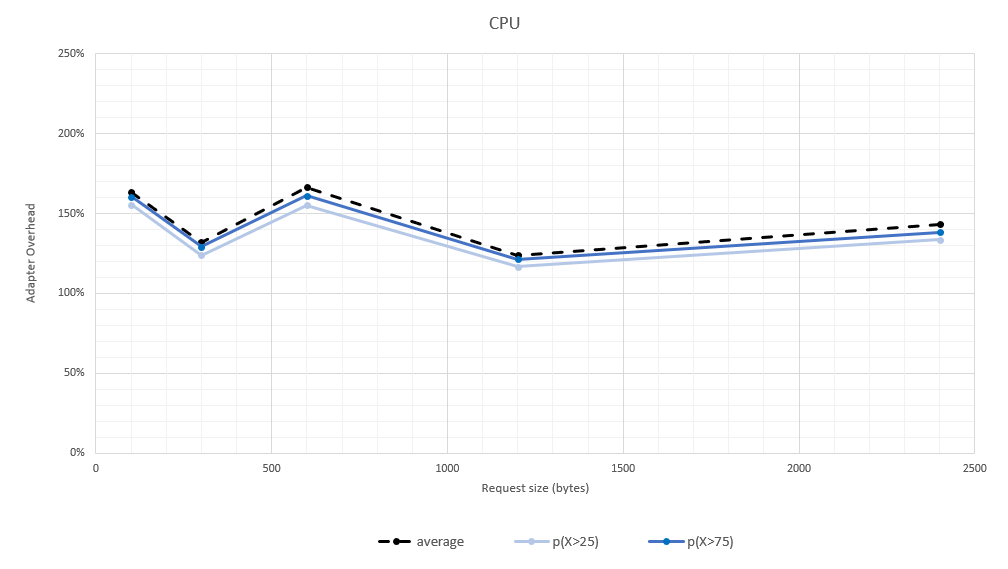
\includegraphics[height=3in]{Results/PtP_Size/Cpu-PtP_Size}
    \caption{Adapter CPU cost in the point-to-point experiment \\\hspace{\textwidth} 480 request/s (arrival rate)}
    \label{fig:payloadCpuPtP}
\end{figure}

\begin{figure}[htbp]
    \centering
    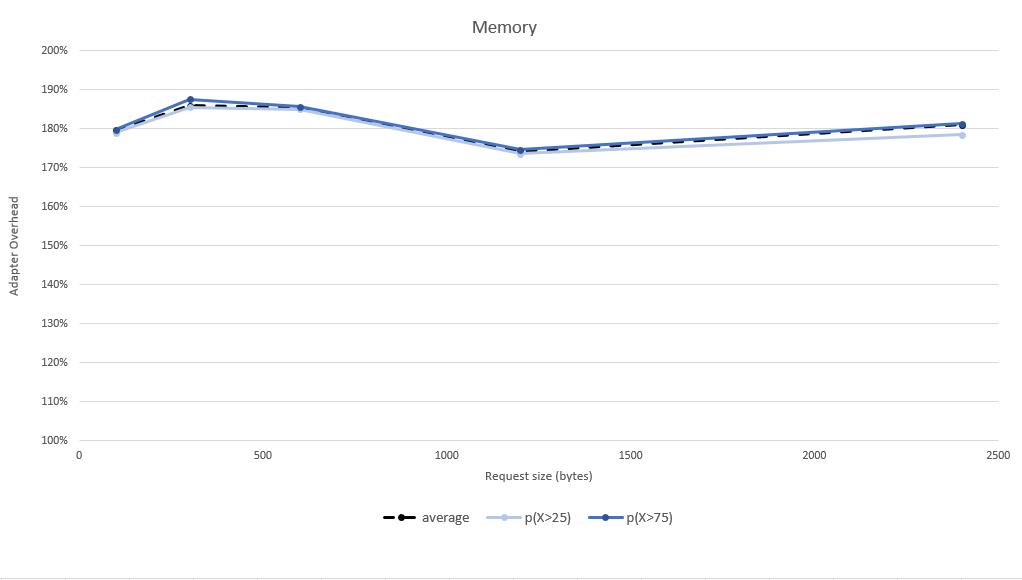
\includegraphics[height=3in]{Results/PtP_Size/Latency-PtP_Size}
    \caption{Adapter Latency cost in the point-to-point experiment \\\hspace{\textwidth} 480 request/s (arrival rate)}
    \label{fig:payloadLatPtP}
\end{figure}

\newpage

\paragraph{Weighted Point to Point}

\begin{figure}[htbp]
    \centering
    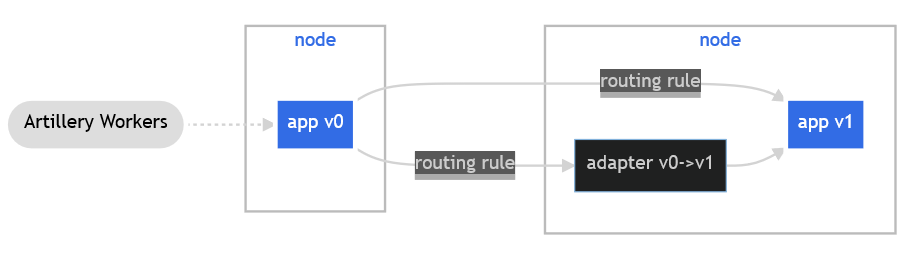
\includegraphics[height=1.8in]{routingExperiment}
    \caption{routing experiment}
    \label{fig:routExp}
\end{figure}

The topology of this experiment is represent in Figure ~\ref{fig:routExp}.
This experiment is also composed by the two microservices, where the first microservice forwards a percentage of its request thorough the adapter
and forwards its remaining requests directly to the other microservice.
The primary goal of this experiment was to see if the adapter overhead is significantly lower in scenarios where only a small percentage of all requests require adaptation.

\paragraph{}

Figure ~\ref{fig:routCpu} depicts the measured CPU cost of the adapter, the horizontal axis represents the percentage of requests that need adaptation, and the vertical axis represents the
CPU cores utilized by the adapter and demo applications.
In this experiment it is expected for the overhead to steadily increase, because as the adapter receives a higher percentage of requests, its request arrival rate will increase, to support higher request rates
the adapter implementation will need to launch more client threads, which consequently increase the consumed CPU resources.

When we compare the first and last data points in Figure ~\ref{fig:routCpu}, we can see that consumed resources have doubled as expected.

In the other data points, the overhead remains relatively constant with a margin of error of 20\%,
this explainable because the default amount of allocated threads by Tomcat (200 threads) is sufficient to handle the arrival rate in these data points.
When 50\% of requests are routed through the adapter, the arrival rate is 240 requests/s, the tomcat thread model uses a thread per request,
consequently 240 threads are necessary to handle the arrival rate, which can be translated to an overhead of 120\%.
The 20\% margin of error in the other data points explainable by the nondeterministic nature of the artillery workers.
The artillery test has two scenarios: one where the worker calls an endpoint that can only be handled by using the adapter, and another in which the adapter is not utilized.
Each scenario weight as set to reflect the corresponding test percentages;
however, the distribution of requests is nondeterministic and will only be equal to the given weights over very long test periods;
the test time for this experiment was set to 5 minutes for each data point.

\paragraph{}

The measured memory overhead of the adapter in this experiment is depicted in Figure ~\ref{fig:routMem}.
It is expected for the overhead to increase linearly with the number of requests, the results obtained confirm our expectations.


\begin{figure}[htbp]
    \centering
    \includegraphics[height=3in]{Results/R/Cpu-R}
    \caption{Adapter CPU cost in the routing experiment \\\hspace{\textwidth} 480 request/s (arrival rate) 100 bytes (payload size)}
    \label{fig:routCpu}
\end{figure}

\begin{figure}[htbp]
    \centering
    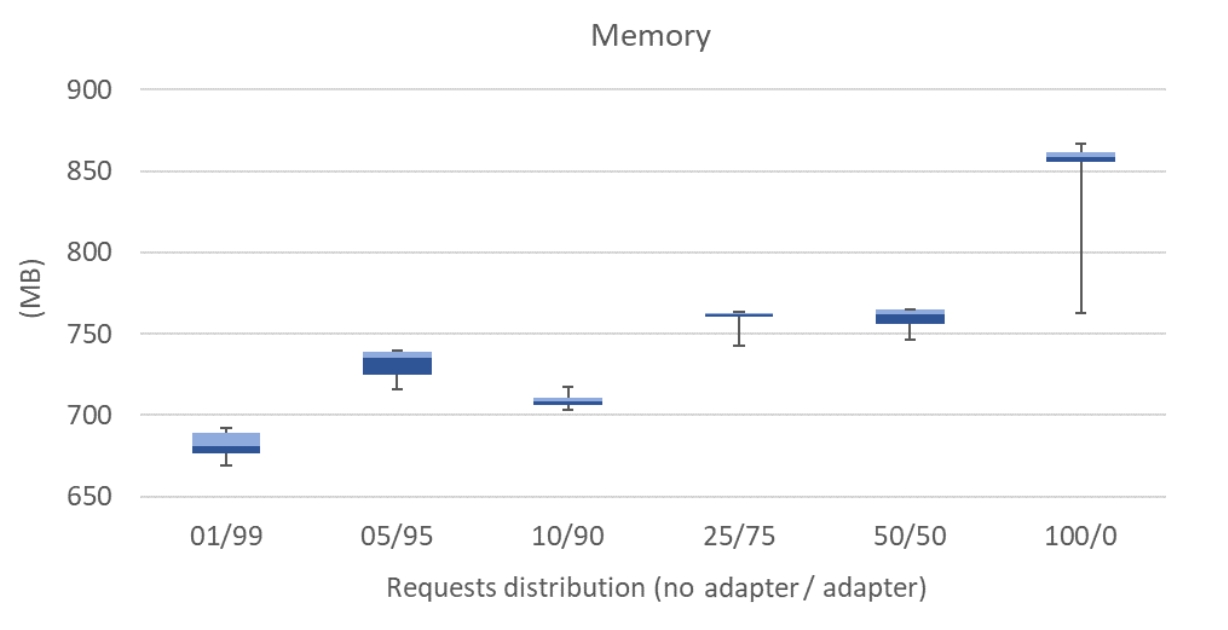
\includegraphics[height=3in]{Results/R/Memory-R}
    \caption{Adapter Memory cost in the routing experiment \\\hspace{\textwidth} 480 request/s (arrival rate) 100 bytes (payload size)}
    \label{fig:routMem}
\end{figure}

\begin{figure}[htbp]
    \centering
    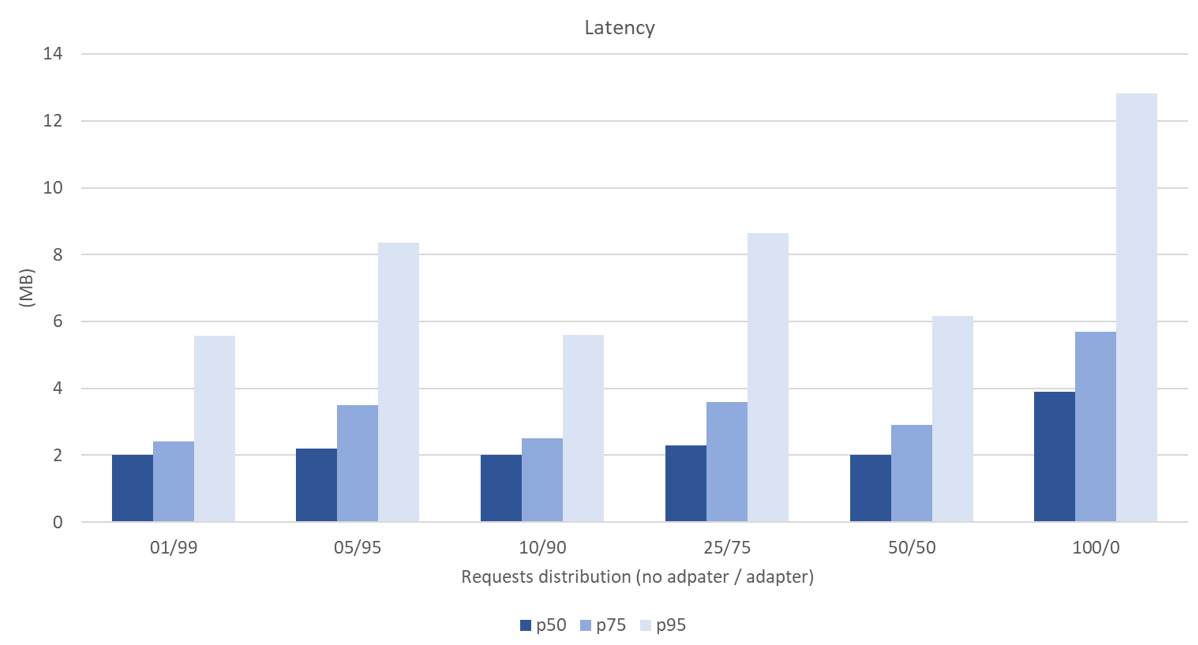
\includegraphics[height=3in]{Results/R/Latency-R}
    \label{fig:gantt}
\end{figure}

\newpage



\paragraph{Bi-partition}

Objective:
Measure Overhead
Measure Consumed Resources
Measure Scalability

\begin{figure}[htbp]
    \centering
    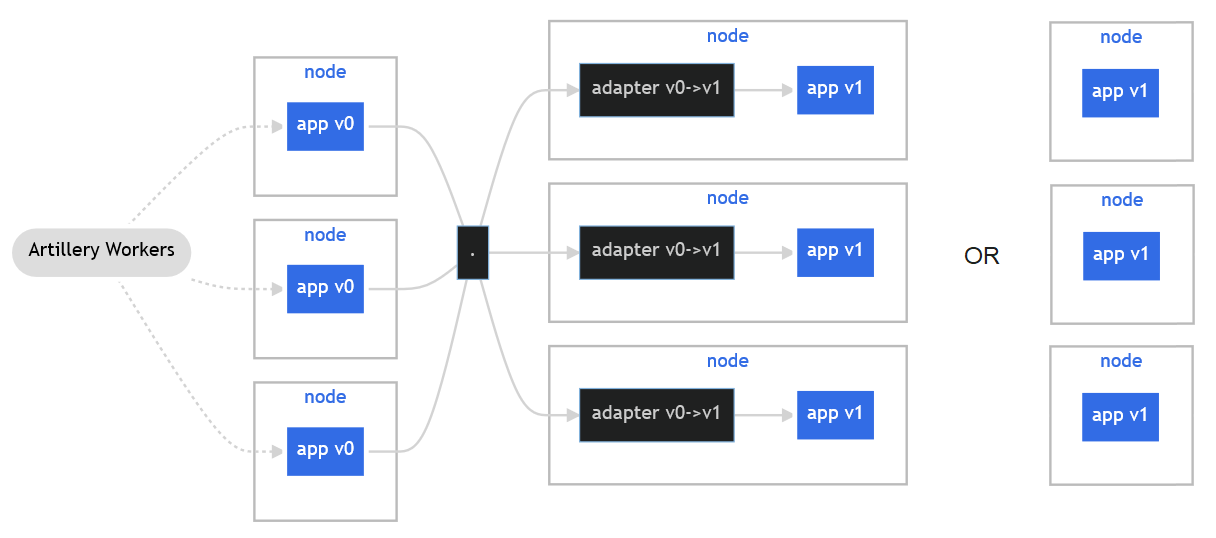
\includegraphics[height=2.7in]{bipartExperiment}
    \caption{bi-partition experiment}
    \label{fig:gantt}
\end{figure}

\begin{figure}[htbp]
    \centering
    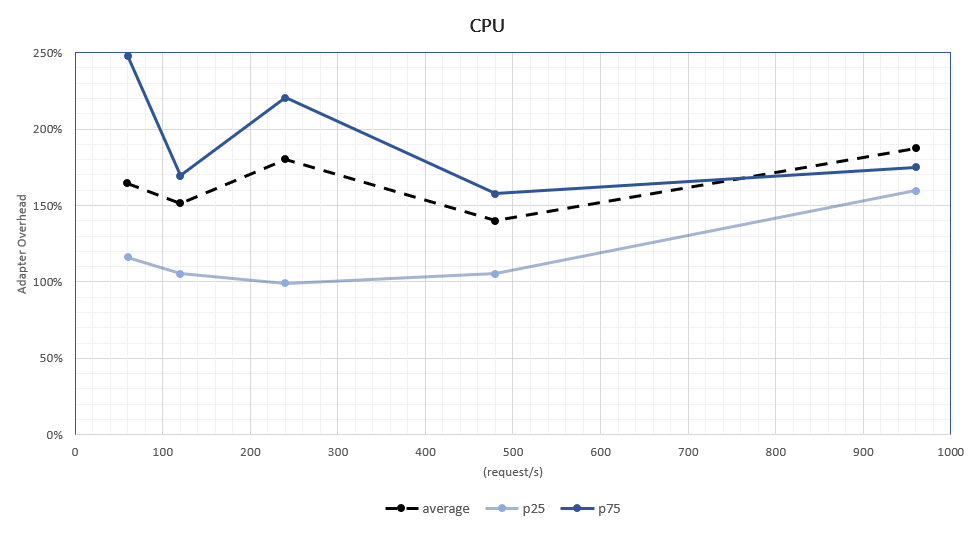
\includegraphics[height=4in]{Results/Bp/Cpu-Bp}
    \label{fig:gantt}
\end{figure}

\begin{figure}[htbp]
    \centering
    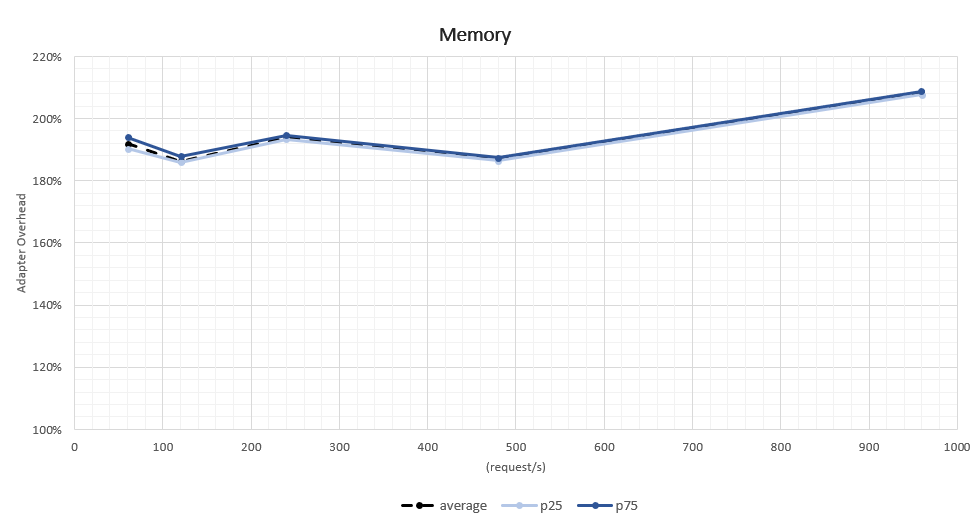
\includegraphics[height=4in]{Results/Bp/Memory-Bp}
    \label{fig:gantt}
\end{figure}

\begin{figure}[htbp]
    \centering
    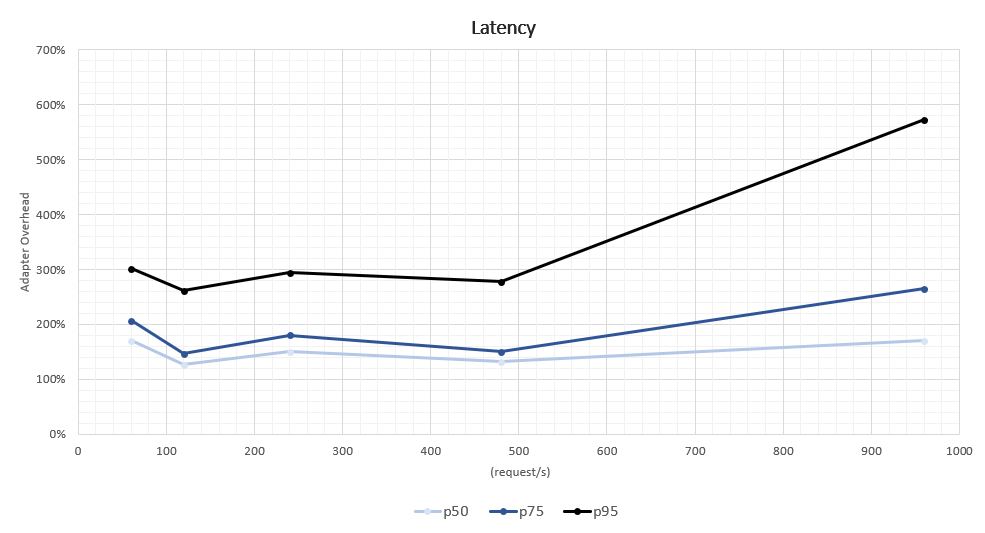
\includegraphics[height=3in]{Results/Bp/Latency-Bp}
    \label{fig:gantt}
\end{figure}